% Task 3 conditional U-Net -- architecture figure (p.1) + hyperparameters (p.2).
% Source of truth: experiment-pipeline/components/models/conditional_unet.py
%                  experiment-pipeline/components/{data,training,losses}/task3.py
%                  experiment-pipeline/configs/task3_unet_pro.toml  (run: task3_unet_finetune_10.pt)
% Shapes verified by forward-hook probe at the inference crop 368x448 (CROP_SIZE in
% experiment-pipeline/scripts/inference_task3_conditional_unet.py).
% Build: latexmk -pdf -interaction=nonstopmode reports/figures/task3_unet_architecture.tex
% Use:   
\includegraphics[page=1,width=\linewidth]{figures/task3_unet_architecture.pdf}  % diagram
%        
\includegraphics[page=2,width=\linewidth]{figures/task3_unet_architecture.pdf}  % hyperparameters
\documentclass[border=8pt,multi=page]{standalone}

\usepackage{lmodern}
\usepackage[T1]{fontenc}
\usepackage{amsmath}
\usepackage{amssymb}
\usepackage{booktabs}
\usepackage{array}
\usepackage{tikz}
\usetikzlibrary{positioning,arrows.meta,calc,fit,backgrounds}

% Categorical hues assigned by role, not by rank. Validated all-pairs (light surface):
% worst CVD dE 9.2 (deutan), worst normal-vision dE 24.0. Aqua sits below 3:1 contrast,
% so the relief rule applies -- every block carries a visible text label.
\definecolor{encblue}{HTML}{2A78D6}    % encoder path
\definecolor{decorange}{HTML}{EB6834}  % decoder path
\definecolor{condaqua}{HTML}{1BAF7A}   % domain conditioning
\definecolor{plumb}{HTML}{6E737B}      % plumbing: pool / upconv / skips (neutral, not a series)
\definecolor{ink}{HTML}{1A1A19}

\tikzset{
  blk/.style   ={rounded corners=2pt, draw, line width=0.9pt, minimum height=9.5mm,
                 align=center, font=\small, text=ink, inner sep=2pt},
  enc/.style   ={blk, draw=encblue,   fill=encblue!8},
  dec/.style   ={blk, draw=decorange, fill=decorange!8},
  bn/.style    ={blk, draw=condaqua,  fill=condaqua!10},
  emb/.style   ={blk, draw=condaqua,  fill=condaqua!14, minimum height=7.5mm, font=\footnotesize},
  io/.style    ={blk, draw=ink!45,    fill=ink!4, minimum height=8mm, font=\footnotesize},
  lay/.style   ={rounded corners=1.5pt, draw=ink!35, fill=white, minimum height=5.2mm,
                 minimum width=34mm, font=\scriptsize, text=ink, inner sep=1pt},
  shp/.style   ={rounded corners=1.5pt, draw=ink!40, fill=white, minimum height=6.4mm,
                 minimum width=31mm, font=\small, text=ink, inner sep=2pt},
  shpz/.style  ={shp, draw=condaqua, fill=condaqua!10},
  shpd/.style  ={shp, draw=decorange, fill=decorange!8},
  sumnode/.style={circle, draw=condaqua, fill=white, line width=0.9pt, inner sep=1pt, font=\small},
  flow/.style  ={-{Stealth[length=2.2mm,width=1.8mm]}, line width=0.9pt, draw=plumb},
  skip/.style  ={-{Stealth[length=2.2mm,width=1.8mm]}, line width=0.9pt, draw=plumb, densely dashed},
  cond/.style  ={-{Stealth[length=2.2mm,width=1.8mm]}, line width=0.9pt, draw=condaqua},
  lead/.style  ={draw=ink!30, line width=0.5pt, densely dotted},
  note/.style  ={font=\scriptsize, text=ink!65, align=left, inner sep=1.5pt},
  tag/.style   ={font=\scriptsize, text=plumb, align=center, inner sep=1.5pt},
  panel/.style ={rounded corners=2.5pt, draw=ink!20, fill=ink!3, inner sep=5pt},
}

\begin{document}

% =====================================================================
% ============================  PAGE 1  ===============================
% =====================================================================
\begin{page}
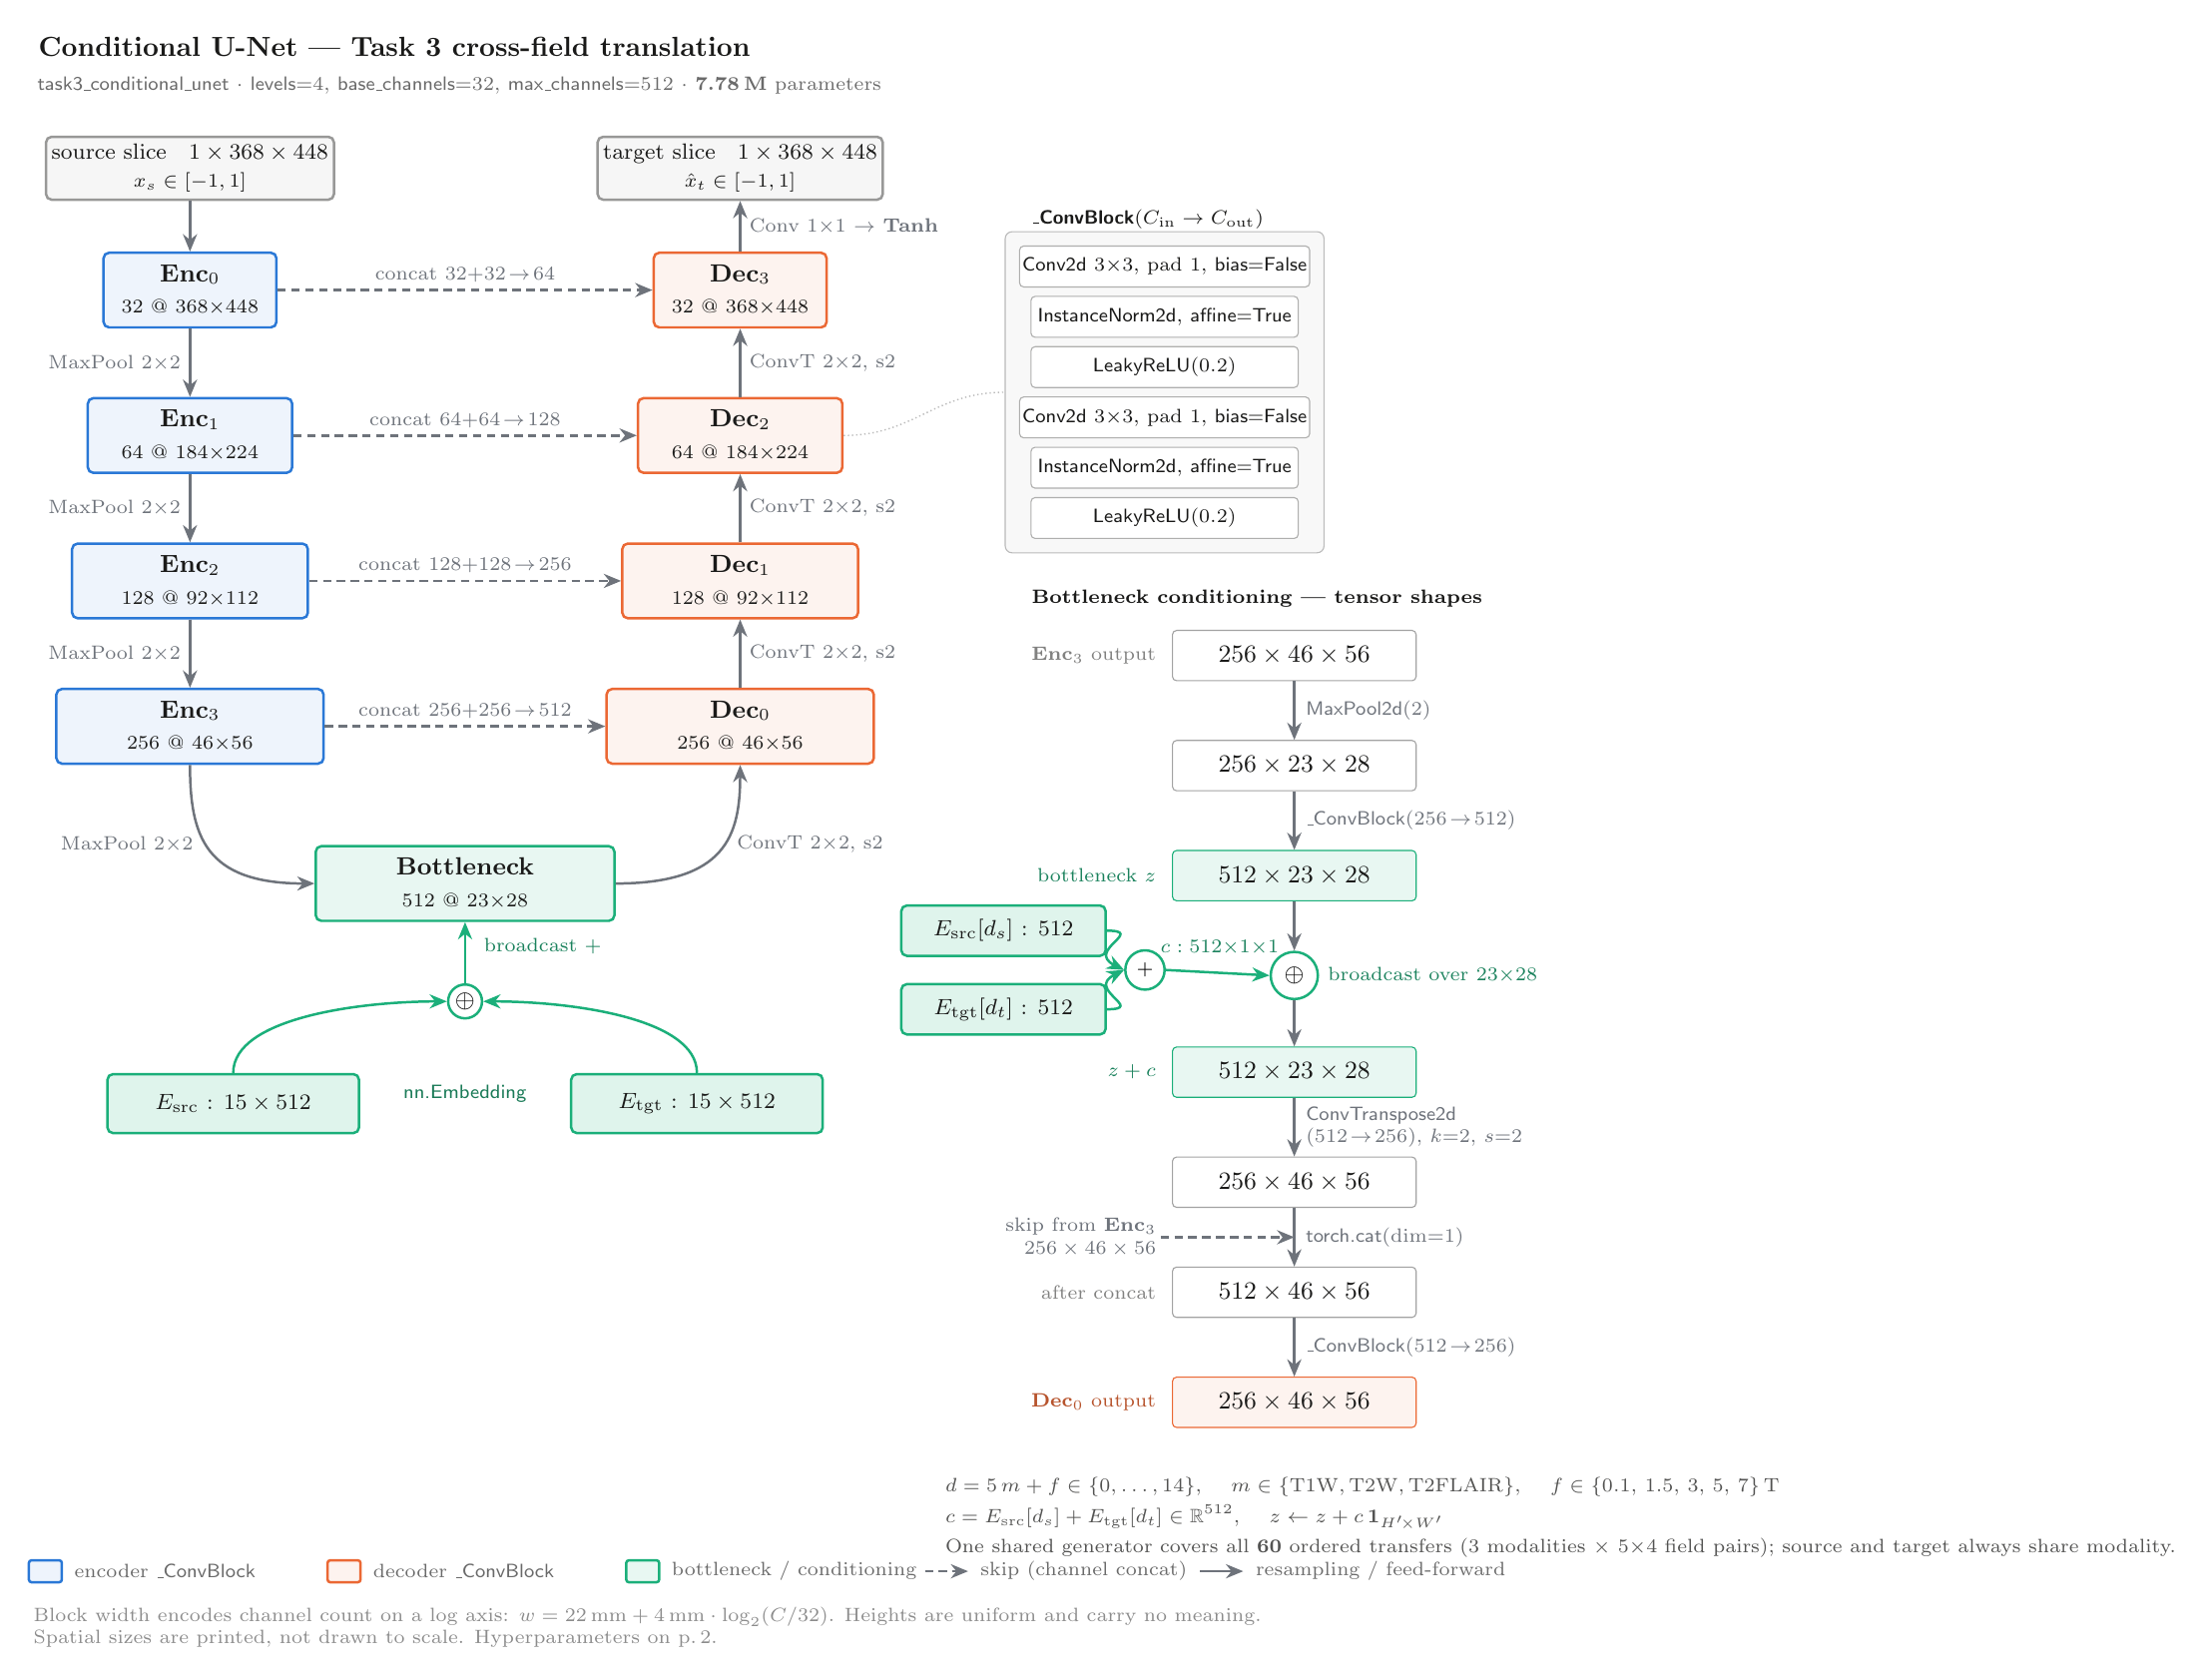
\begin{tikzpicture}[x=1cm, y=1cm]

% ------------------------- title -------------------------
\node[anchor=west, font=\bfseries, text=ink] at (-2.05, 3.10)
     {Conditional U-Net --- Task 3 cross-field translation};
\node[anchor=west, note] at (-2.0, 2.60)
     {\textsf{task3\_conditional\_unet} $\cdot$ \textsf{levels}=4, \textsf{base\_channels}=32,
      \textsf{max\_channels}=512 $\cdot$ \textbf{7.78\,M} parameters};

% ------------------------- I/O -------------------------
\node[io, minimum width=30mm] (IN)  at (0,   1.55)
     {source slice \; $1\times368\times448$\\[0.5pt]\scriptsize $x_s \in [-1,1]$};
\node[io, minimum width=30mm] (OUT) at (7.0, 1.55)
     {target slice \; $1\times368\times448$\\[0.5pt]\scriptsize $\hat{x}_t \in [-1,1]$};

% ------------------------- encoder -------------------------
% Box width = 22mm + 4mm * log2(C/32)  -- i.e. width is linear in log2(channels).
\node[enc, minimum width=22mm] (E0) at (0, 0)     {\textbf{Enc}$_0$\\[0.5pt]\scriptsize 32 @ $368{\times}448$};
\node[enc, minimum width=26mm] (E1) at (0,-1.85)  {\textbf{Enc}$_1$\\[0.5pt]\scriptsize 64 @ $184{\times}224$};
\node[enc, minimum width=30mm] (E2) at (0,-3.70)  {\textbf{Enc}$_2$\\[0.5pt]\scriptsize 128 @ $92{\times}112$};
\node[enc, minimum width=34mm] (E3) at (0,-5.55)  {\textbf{Enc}$_3$\\[0.5pt]\scriptsize 256 @ $46{\times}56$};

% ------------------------- bottleneck -------------------------
\node[bn, minimum width=38mm] (BN) at (3.5,-7.55) {\textbf{Bottleneck}\\[0.5pt]\scriptsize 512 @ $23{\times}28$};

% ------------------------- decoder -------------------------
\node[dec, minimum width=34mm] (D3) at (7.0,-5.55) {\textbf{Dec}$_0$\\[0.5pt]\scriptsize 256 @ $46{\times}56$};
\node[dec, minimum width=30mm] (D2) at (7.0,-3.70) {\textbf{Dec}$_1$\\[0.5pt]\scriptsize 128 @ $92{\times}112$};
\node[dec, minimum width=26mm] (D1) at (7.0,-1.85) {\textbf{Dec}$_2$\\[0.5pt]\scriptsize 64 @ $184{\times}224$};
\node[dec, minimum width=22mm] (D0) at (7.0, 0)    {\textbf{Dec}$_3$\\[0.5pt]\scriptsize 32 @ $368{\times}448$};

% ------------------------- flow: down -------------------------
\draw[flow] (IN) -- (E0);
\draw[flow] (E0) -- node[tag, left=0.5mm] {MaxPool $2{\times}2$} (E1);
\draw[flow] (E1) -- node[tag, left=0.5mm] {MaxPool $2{\times}2$} (E2);
\draw[flow] (E2) -- node[tag, left=0.5mm] {MaxPool $2{\times}2$} (E3);
\draw[flow] (E3.south) .. controls +(0,-0.9) and +(-1.4,0) .. (BN.west);
\node[tag, anchor=east] at (0.10,-7.05) {MaxPool $2{\times}2$};

% ------------------------- flow: up -------------------------
\draw[flow] (BN.east) .. controls +(1.4,0) and +(0,-0.9) .. (D3.south);
\node[tag, anchor=west] at (6.90,-7.05) {ConvT $2{\times}2$, s2};
\draw[flow] (D3) -- node[tag, right=0.5mm] {ConvT $2{\times}2$, s2} (D2);
\draw[flow] (D2) -- node[tag, right=0.5mm] {ConvT $2{\times}2$, s2} (D1);
\draw[flow] (D1) -- node[tag, right=0.5mm] {ConvT $2{\times}2$, s2} (D0);
\draw[flow] (D0) -- node[tag, right=0.5mm] {Conv $1{\times}1$ $\to$ \textbf{Tanh}} (OUT);

% ------------------------- skip connections -------------------------
\draw[skip] (E0.east) -- node[tag, above=0.3mm] {concat $32{+}32\!\to\!64$}  (D0.west);
\draw[skip] (E1.east) -- node[tag, above=0.3mm] {concat $64{+}64\!\to\!128$} (D1.west);
\draw[skip] (E2.east) -- node[tag, above=0.3mm] {concat $128{+}128\!\to\!256$} (D2.west);
\draw[skip] (E3.east) -- node[tag, above=0.3mm] {concat $256{+}256\!\to\!512$} (D3.west);

% ------------------------- conditioning -------------------------
\node[sumnode] (SUM) at (3.5,-9.05) {$\oplus$};
\node[emb, minimum width=32mm] (ES) at (0.55,-10.35) {$E_{\mathrm{src}}$ : $15\times512$};
\node[emb, minimum width=32mm] (ET) at (6.45,-10.35) {$E_{\mathrm{tgt}}$ : $15\times512$};
\node[note, anchor=north, text=condaqua!65!ink] at (3.5,-10.05) {\textsf{nn.Embedding}};

\draw[cond] (ES.north) .. controls +(0,0.7) and +(-1.1,0) .. (SUM.west);
\draw[cond] (ET.north) .. controls +(0,0.7) and +(1.1,0)  .. (SUM.east);
\draw[cond] (SUM.north) -- (BN.south);
\node[tag, anchor=west, text=condaqua!70!ink] at (3.68,-8.35) {broadcast $+$};

% ------------------------- \_ConvBlock inset -------------------------
\node[lay] (L1) at (12.4, 0.30) {\textsf{Conv2d} $3{\times}3$, pad 1, \textsf{bias=False}};
\node[lay] (L2) at (12.4,-0.34) {\textsf{InstanceNorm2d}, \textsf{affine=True}};
\node[lay] (L3) at (12.4,-0.98) {\textsf{LeakyReLU}$(0.2)$};
\node[lay] (L4) at (12.4,-1.62) {\textsf{Conv2d} $3{\times}3$, pad 1, \textsf{bias=False}};
\node[lay] (L5) at (12.4,-2.26) {\textsf{InstanceNorm2d}, \textsf{affine=True}};
\node[lay] (L6) at (12.4,-2.90) {\textsf{LeakyReLU}$(0.2)$};
\node[note, anchor=south west, font=\scriptsize\bfseries, text=ink]
      at (10.65, 0.72) {\textsf{\_ConvBlock}$(C_{\mathrm{in}} \to C_{\mathrm{out}})$};
\begin{scope}[on background layer]
  \node[panel, fit=(L1)(L6), draw=ink!30, fill=ink!3] (INSET) {};
\end{scope}
\draw[lead] (D1.east) .. controls +(0.9,0) and +(-0.9,0) .. (INSET.west);

% ---------- bottleneck conditioning: shape flow (right column) -------
\node[note, anchor=north west, font=\scriptsize\bfseries, text=ink] at (10.65,-3.75)
      {Bottleneck conditioning --- tensor shapes};

\node[shp]  (T1) at (14.05,-4.65) {$256 \times 46 \times 56$};
\node[shp]  (T2) at (14.05,-6.05) {$256 \times 23 \times 28$};
\node[shpz] (T3) at (14.05,-7.45) {$512 \times 23 \times 28$};
\node[sumnode, minimum size=6mm] (PLUS) at (14.05,-8.72) {$\oplus$};
\node[shpz] (T4) at (14.05,-9.95) {$512 \times 23 \times 28$};
\node[shp]  (T5) at (14.05,-11.35) {$256 \times 46 \times 56$};
\node[shp]  (T6) at (14.05,-12.75) {$512 \times 46 \times 56$};
\node[shpd] (T7) at (14.05,-14.15) {$256 \times 46 \times 56$};

\draw[flow] (T1) -- node[tag, right=0.8mm] {\textsf{MaxPool2d}(2)} (T2);
\draw[flow] (T2) -- node[tag, right=0.8mm] {\textsf{\_ConvBlock}$(256\!\to\!512)$} (T3);
\draw[flow] (T3) -- (PLUS);
\draw[flow] (PLUS) -- (T4);
\draw[flow] (T4) -- node[tag, right=0.8mm, align=left] {\textsf{ConvTranspose2d}\\$(512\!\to\!256)$, $k{=}2$, $s{=}2$} (T5);
\draw[flow] (T5) -- node[tag, right=0.8mm] {\textsf{torch.cat}(dim=1)} (T6);
\draw[flow] (T6) -- node[tag, right=0.8mm] {\textsf{\_ConvBlock}$(512\!\to\!256)$} (T7);

% row labels on the left of the ladder
\node[note, anchor=east, text=ink!55] at (12.35,-4.65) {\textbf{Enc}$_3$ output};
\node[note, anchor=east, text=condaqua!70!ink] at (12.35,-7.45) {bottleneck $z$};
\node[note, anchor=east, text=condaqua!70!ink] at (12.35,-9.95) {$z + c$};
\node[note, anchor=east, text=ink!55] at (12.35,-12.75) {after concat};
\node[note, anchor=east, text=decorange!75!ink] at (12.35,-14.15) {\textbf{Dec}$_0$ output};

% --- embedding branch feeding the broadcast add ---
\node[emb, minimum width=26mm, minimum height=6.4mm] (BES) at (10.35,-8.15)
     {$E_{\mathrm{src}}[d_s]$ : $512$};
\node[emb, minimum width=26mm, minimum height=6.4mm] (BET) at (10.35,-9.15)
     {$E_{\mathrm{tgt}}[d_t]$ : $512$};
\node[sumnode, minimum size=5mm] (BSUM) at (12.15,-8.65) {\scriptsize$+$};
\draw[cond] (BES.east) .. controls +(0.5,0) and +(-0.5,0.25) .. (BSUM.west);
\draw[cond] (BET.east) .. controls +(0.5,0) and +(-0.5,-0.25) .. (BSUM.west);
\draw[cond] (BSUM.east) -- (PLUS.west);
\node[tag, anchor=south, text=condaqua!70!ink] at (13.10,-8.52) {$c: 512{\times}1{\times}1$};
\node[tag, anchor=west, text=condaqua!70!ink] at (14.42,-8.72) {broadcast over $23{\times}28$};

% --- skip feeding the concat ---
\node[note, anchor=east, text=plumb, align=right] (SKLAB) at (12.35,-12.05)
     {skip from \textbf{Enc}$_3$\\$256\times46\times56$};
\draw[skip] (SKLAB.east) .. controls +(0.6,0) and +(-0.9,0) .. ($(T5)!0.5!(T6)$);

% --- the one formula kept on this page ---
\node[note, anchor=north west, text=ink!75] at (9.55,-15.05)
     {$d = 5\,m + f \in \{0,\dots,14\}$, \quad
      $m \in \{\text{T1W},\text{T2W},\text{T2FLAIR}\}$, \quad
      $f \in \{0.1,\,1.5,\,3,\,5,\,7\}\,$T\\[3pt]
      $c = E_{\mathrm{src}}[d_s] + E_{\mathrm{tgt}}[d_t] \in \mathbb{R}^{512}$, \quad
      $z \leftarrow z + c\,\mathbf{1}_{H'\!\times W'}$\\[3pt]
      One shared generator covers all \textbf{60} ordered transfers
      (3 modalities $\times$ $5{\times}4$ field pairs); source and target always share modality.};

% ------------------------- legend -------------------------
\draw[fill=encblue!8,   draw=encblue,   line width=0.9pt, rounded corners=1pt] (-2.05,-16.44) rectangle ++(0.42,0.28);
\node[note, anchor=west] at (-1.53,-16.30) {encoder \textsf{\_ConvBlock}};
\draw[fill=decorange!8, draw=decorange, line width=0.9pt, rounded corners=1pt] (1.75,-16.44) rectangle ++(0.42,0.28);
\node[note, anchor=west] at (2.27,-16.30) {decoder \textsf{\_ConvBlock}};
\draw[fill=condaqua!10, draw=condaqua,  line width=0.9pt, rounded corners=1pt] (5.55,-16.44) rectangle ++(0.42,0.28);
\node[note, anchor=west] at (6.07,-16.30) {bottleneck / conditioning};
\draw[skip] (9.35,-16.30) -- ++(0.55,0);
\node[note, anchor=west] at (10.0,-16.30) {skip (channel concat)};
\draw[flow] (12.85,-16.30) -- ++(0.55,0);
\node[note, anchor=west] at (13.5,-16.30) {resampling / feed-forward};
\node[note, anchor=north west, text=ink!50] at (-2.05,-16.70)
     {Block width encodes channel count on a log axis: $w = 22\,\mathrm{mm} + 4\,\mathrm{mm}\cdot\log_2(C/32)$. Heights are uniform and carry no meaning.\\
      Spatial sizes are printed, not drawn to scale. Hyperparameters on p.\,2.};

\end{tikzpicture}
\end{page}

% =====================================================================
% ============================  PAGE 2  ===============================
% =====================================================================
\begin{page}
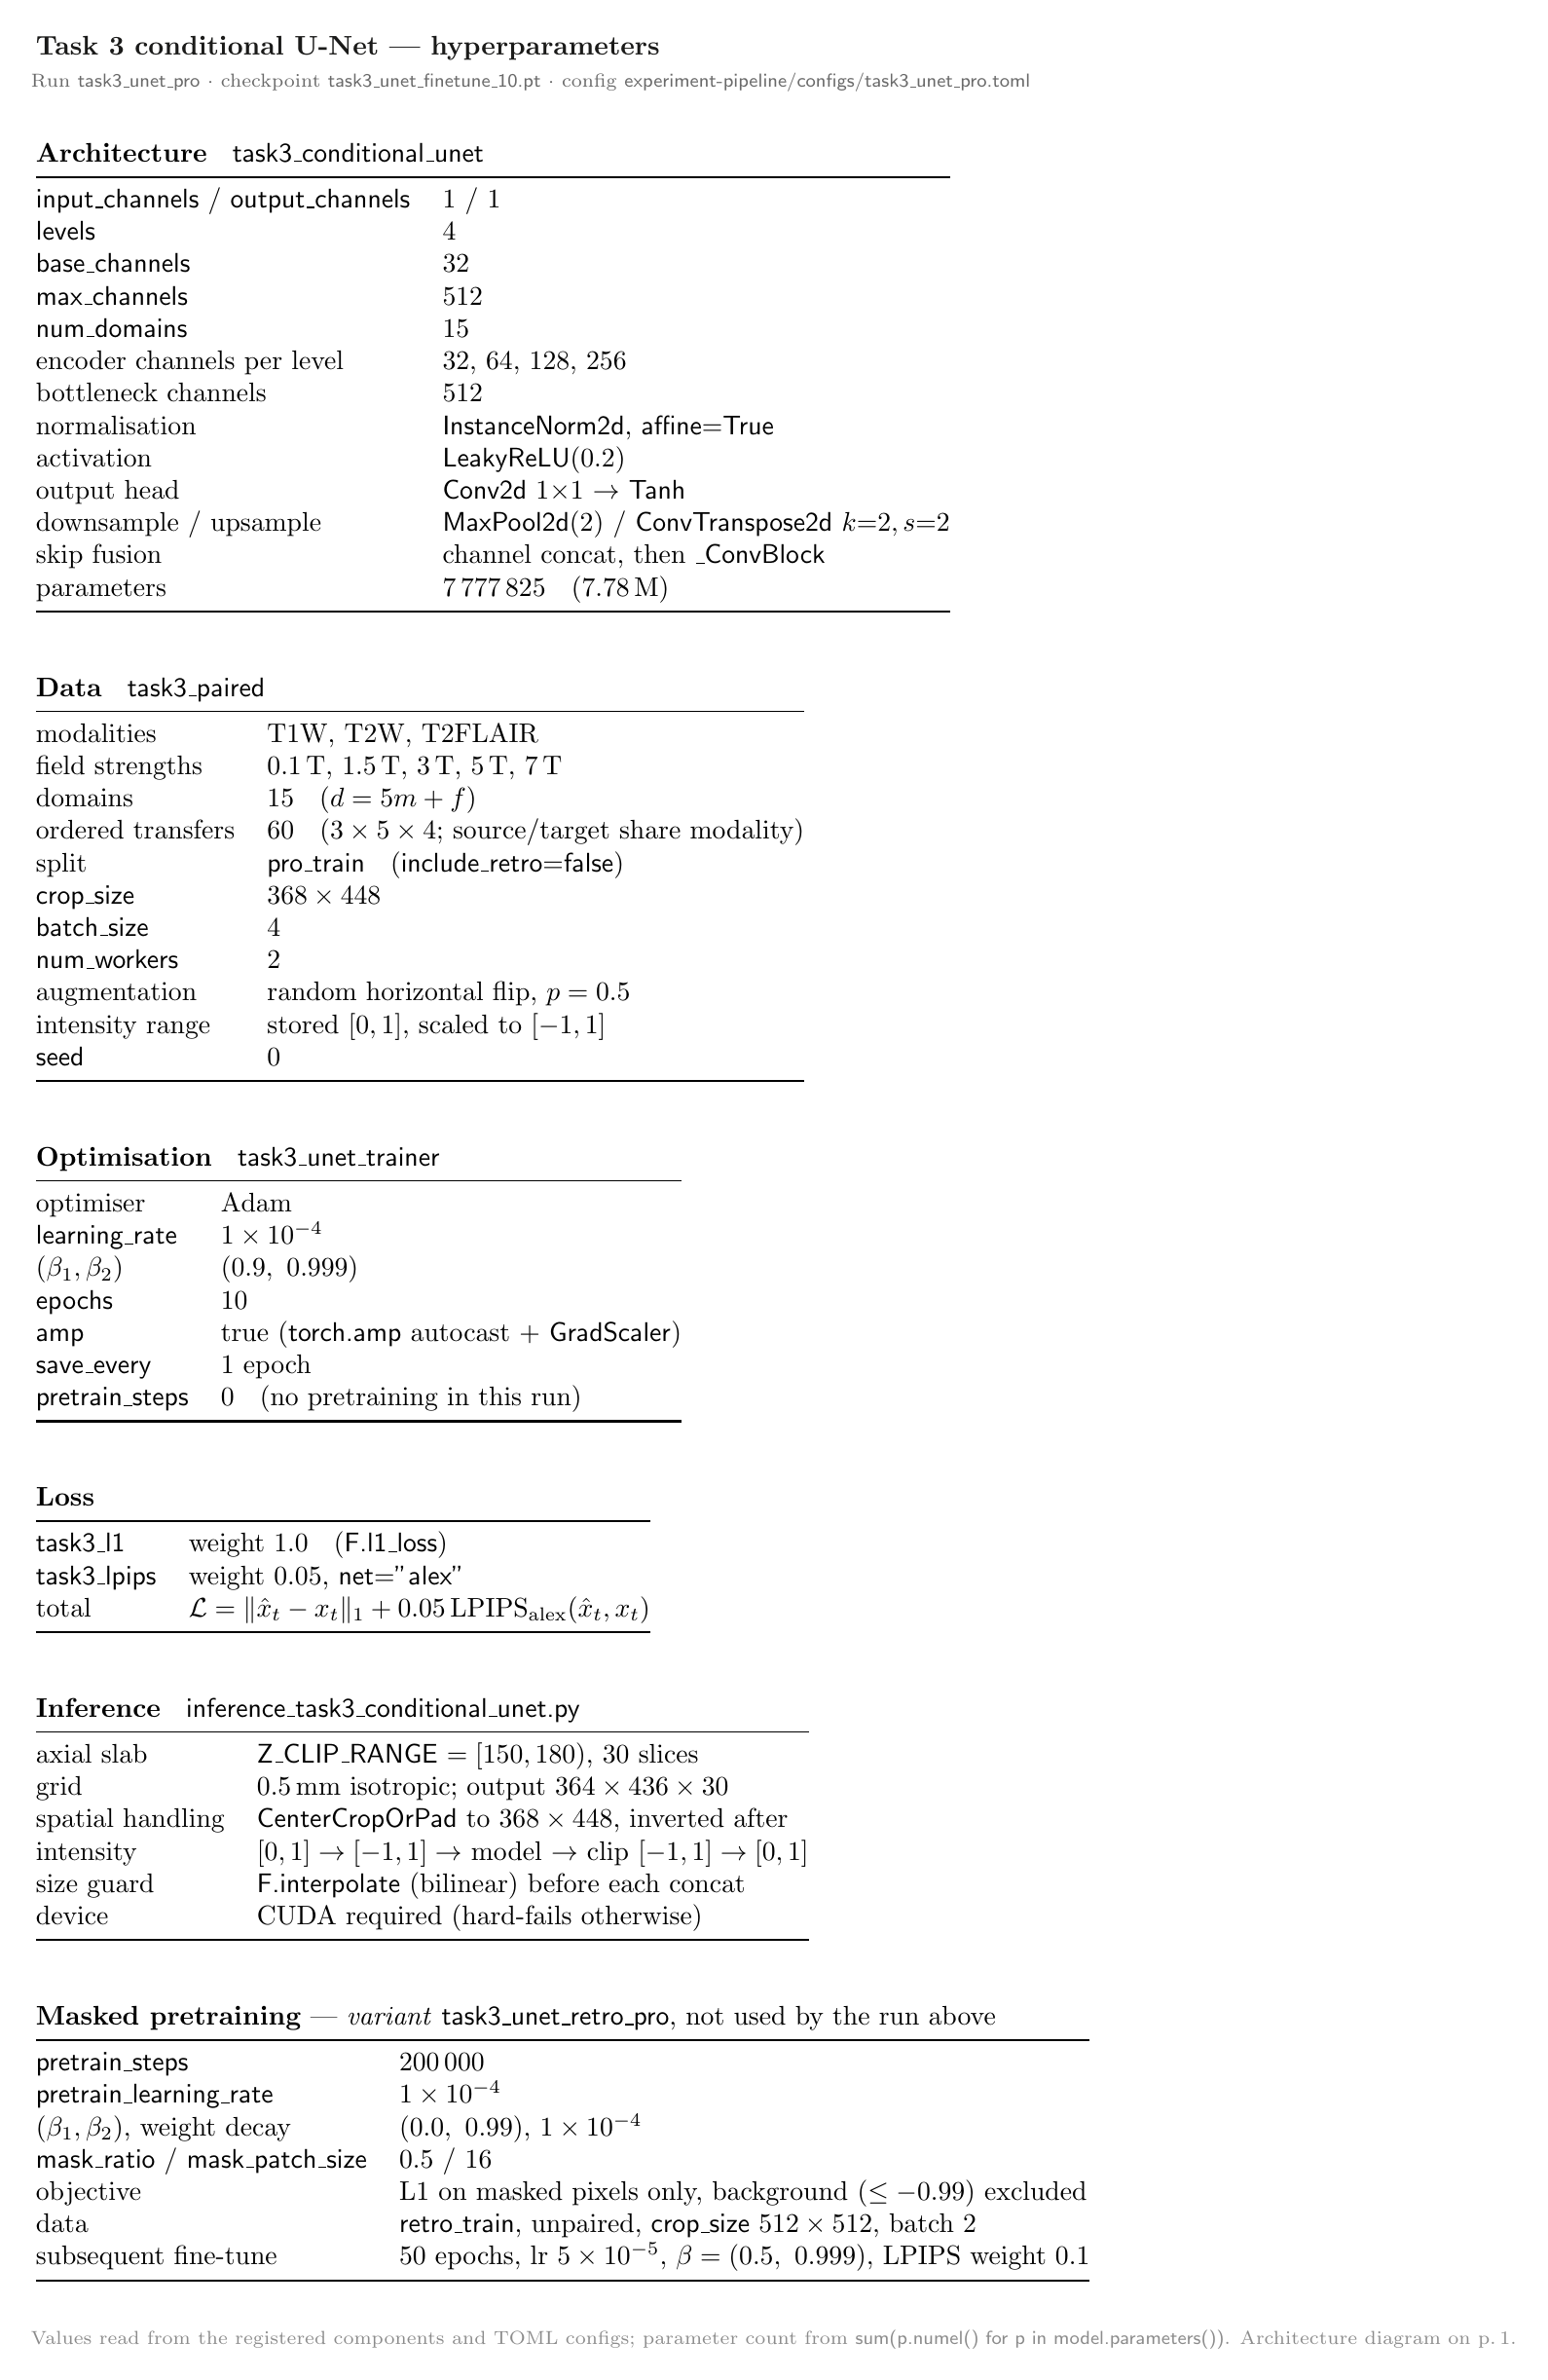
\begin{tikzpicture}[x=1cm, y=1cm]
\node[anchor=north west, font=\bfseries, text=ink] (TT) at (0,0)
     {Task 3 conditional U-Net --- hyperparameters};
\node[anchor=north west, note] (TS) at (0,-0.55)
     {Run \textsf{task3\_unet\_pro} $\cdot$ checkpoint \textsf{task3\_unet\_finetune\_10.pt} $\cdot$
      config \textsf{experiment-pipeline/configs/task3\_unet\_pro.toml}};

% ---------------- column 1 ----------------
\node[anchor=north west] (C1A) at (0,-1.35) {%
\begin{tabular}{@{}l l@{}}
\multicolumn{2}{@{}l}{\textbf{Architecture} \; \textsf{task3\_conditional\_unet}}\\
\midrule
\textsf{input\_channels} / \textsf{output\_channels} & 1 / 1 \\
\textsf{levels}                        & 4 \\
\textsf{base\_channels}                & 32 \\
\textsf{max\_channels}                 & 512 \\
\textsf{num\_domains}                  & 15 \\
encoder channels per level             & 32, 64, 128, 256 \\
bottleneck channels                    & 512 \\
normalisation                          & \textsf{InstanceNorm2d}, \textsf{affine=True} \\
activation                             & \textsf{LeakyReLU}$(0.2)$ \\
output head                            & \textsf{Conv2d} $1{\times}1$ $\to$ \textsf{Tanh} \\
downsample / upsample                  & \textsf{MaxPool2d}(2) / \textsf{ConvTranspose2d} $k{=}2,s{=}2$ \\
skip fusion                            & channel concat, then \textsf{\_ConvBlock} \\
parameters                             & 7\,777\,825 \; (7.78\,M) \\
\bottomrule
\end{tabular}};

\node[anchor=north west] (C1B) at ($(C1A.south west)+(0,-0.55)$) {%
\begin{tabular}{@{}l l@{}}
\multicolumn{2}{@{}l}{\textbf{Data} \; \textsf{task3\_paired}}\\
\midrule
modalities            & T1W, T2W, T2FLAIR \\
field strengths       & 0.1\,T, 1.5\,T, 3\,T, 5\,T, 7\,T \\
domains               & 15 \; $(d = 5m + f)$ \\
ordered transfers     & 60 \; ($3 \times 5 \times 4$; source/target share modality) \\
split                 & \textsf{pro\_train} \; (\textsf{include\_retro=false}) \\
\textsf{crop\_size}   & $368 \times 448$ \\
\textsf{batch\_size}  & 4 \\
\textsf{num\_workers} & 2 \\
augmentation          & random horizontal flip, $p = 0.5$ \\
intensity range       & stored $[0,1]$, scaled to $[-1,1]$ \\
\textsf{seed}         & 0 \\
\bottomrule
\end{tabular}};

\node[anchor=north west] (C2A) at ($(C1B.south west)+(0,-0.55)$) {%
\begin{tabular}{@{}l l@{}}
\multicolumn{2}{@{}l}{\textbf{Optimisation} \; \textsf{task3\_unet\_trainer}}\\
\midrule
optimiser             & Adam \\
\textsf{learning\_rate} & $1\times10^{-4}$ \\
$(\beta_1, \beta_2)$  & $(0.9,\ 0.999)$ \\
\textsf{epochs}       & 10 \\
\textsf{amp}          & true (\textsf{torch.amp} autocast + \textsf{GradScaler}) \\
\textsf{save\_every}  & 1 epoch \\
\textsf{pretrain\_steps} & 0 \; (no pretraining in this run) \\
\bottomrule
\end{tabular}};

\node[anchor=north west] (C2B) at ($(C2A.south west)+(0,-0.55)$) {%
\begin{tabular}{@{}l l@{}}
\multicolumn{2}{@{}l}{\textbf{Loss}}\\
\midrule
\textsf{task3\_l1}    & weight 1.0 \; (\textsf{F.l1\_loss}) \\
\textsf{task3\_lpips} & weight 0.05, \textsf{net="alex"} \\
total                 & $\mathcal{L} = \lVert \hat{x}_t - x_t \rVert_1 + 0.05\,\mathrm{LPIPS}_{\text{alex}}(\hat{x}_t, x_t)$ \\
\bottomrule
\end{tabular}};

\node[anchor=north west] (C2C) at ($(C2B.south west)+(0,-0.55)$) {%
\begin{tabular}{@{}l l@{}}
\multicolumn{2}{@{}l}{\textbf{Inference} \; \textsf{inference\_task3\_conditional\_unet.py}}\\
\midrule
axial slab            & \textsf{Z\_CLIP\_RANGE} $= [150, 180)$, 30 slices \\
grid                  & 0.5\,mm isotropic; output $364 \times 436 \times 30$ \\
spatial handling      & \textsf{CenterCropOrPad} to $368 \times 448$, inverted after \\
intensity             & $[0,1] \to [-1,1] \to$ model $\to$ clip $[-1,1] \to [0,1]$ \\
size guard            & \textsf{F.interpolate} (bilinear) before each concat \\
device                & CUDA required (hard-fails otherwise) \\
\bottomrule
\end{tabular}};

\node[anchor=north west] (BOT) at ($(C2C.south west)+(0,-0.55)$) {%
\begin{tabular}{@{}l l@{}}
\multicolumn{2}{@{}l}{\textbf{Masked pretraining} --- \emph{variant} \textsf{task3\_unet\_retro\_pro}, not used by the run above}\\
\midrule
\textsf{pretrain\_steps}                    & 200\,000 \\
\textsf{pretrain\_learning\_rate}           & $1\times10^{-4}$ \\
$(\beta_1, \beta_2)$, weight decay          & $(0.0,\ 0.99)$, $1\times10^{-4}$ \\
\textsf{mask\_ratio} / \textsf{mask\_patch\_size} & 0.5 / 16 \\
objective                                   & L1 on masked pixels only, background ($\leq -0.99$) excluded \\
data                                        & \textsf{retro\_train}, unpaired, \textsf{crop\_size} $512\times512$, batch 2 \\
subsequent fine-tune                        & 50 epochs, lr $5\times10^{-5}$, $\beta = (0.5,\ 0.999)$, LPIPS weight 0.1 \\
\bottomrule
\end{tabular}};

\node[anchor=north west, note, text=ink!50] at ($(BOT.south west)+(0,-0.45)$)
     {Values read from the registered components and TOML configs; parameter count from
      \textsf{sum(p.numel() for p in model.parameters())}. Architecture diagram on p.\,1.};
\end{tikzpicture}
\end{page}

\end{document}
